%%%%%%%%%%%%%%%%%%%%%%%%%%%%%%%%%%%%%%%%%
% Beamer Presentation
% LaTeX Template
% Version 1.0 (10/11/12)
%
% This template has been downloaded from:
% http://www.LaTeXTemplates.com
%
% License:
% CC BY-NC-SA 3.0 (http://creativecommons.org/licenses/by-nc-sa/3.0/)
%
%%%%%%%%%%%%%%%%%%%%%%%%%%%%%%%%%%%%%%%%%

%----------------------------------------------------------------------------------------
%	PACKAGES AND THEMES
%----------------------------------------------------------------------------------------

%\documentclass[UTF8,aspectratio=169,14pt]{ctexbeamer}
\documentclass[UTF8,aspectratio=169]{ctexbeamer}
\usepackage{hyperref}
\hypersetup{
	colorlinks=true,
	linkcolor=red,
	anchorcolor=blue,
	citecolor=green
}

\mode<presentation> {
	
	% The Beamer class comes with a number of default slide themes
	% which change the colors and layouts of slides. Below this is a list
	% of all the themes, uncomment each in turn to see what they look like.
	
	%\usetheme{default}
	%\usetheme{AnnArbor}
	%\usetheme{Antibes}
	%\usetheme{Bergen}
	%\usetheme{Berkeley}
	%\usetheme{Berlin}
	%\usetheme{Boadilla}
	%\usetheme{CambridgeUS}
	%\usetheme{Copenhagen}
	%\usetheme{Darmstadt}
	%\usetheme{Dresden}
	%\usetheme{Frankfurt}
	%\usetheme{Goettingen}
	%\usetheme{Hannover}
	%\usetheme{Ilmenau}
	%\usetheme{JuanLesPins}
	%\usetheme{Luebeck}
	\usetheme{Madrid}
	%\usetheme{Malmoe}
	%\usetheme{Marburg}
	%\usetheme{Montpellier}
	%\usetheme{PaloAlto}
	%\usetheme{Pittsburgh}
	%\usetheme{Rochester}
	%\usetheme{Singapore}
	%\usetheme{Szeged}
	%\usetheme{Warsaw}
	
	% As well as themes, the Beamer class has a number of color themes
	% for any slide theme. Uncomment each of these in turn to see how it
	% changes the colors of your current slide theme.
	
	%\usecolortheme{albatross}
	%\usecolortheme{beaver}
	%\usecolortheme{beetle}
	%\usecolortheme{crane}
	%\usecolortheme{dolphin}
	%\usecolortheme{dove}
	%\usecolortheme{fly}
	%\usecolortheme{lily}
	%\usecolortheme{orchid}
	%\usecolortheme{rose}
	%\usecolortheme{seagull}
	%\usecolortheme{seahorse}
	%\usecolortheme{whale}
	%\usecolortheme{wolverine}
	
	%\setbeamertemplate{footline} % To remove the footer line in all slides uncomment this line
	%\setbeamertemplate{footline}[page number] % To replace the footer line in all slides with a simple slide count uncomment this line
	
	%\setbeamertemplate{navigation symbols}{} % To remove the navigation symbols from the bottom of all slides uncomment this line
}

\usepackage{graphicx} % Allows including images
\graphicspath{{./figs/}}
\usepackage{booktabs} % Allows the use of \toprule, \midrule and \bottomrule in tables
\usepackage{longtable}
\usepackage{listings}
\usepackage{xcolor}
\lstset{numbers=left, %设置行号位置
	numberstyle=\tiny, %设置行号大小
	keywordstyle=\color{blue}, %设置关键字颜色
	commentstyle=\color[cmyk]{1,0,1,0}, %设置注释颜色
	frame=single, %设置边框格式
	escapeinside=``, %逃逸字符(1左面的键),用于显示中文
	%breaklines, %自动折行
	extendedchars=false, %解决代码跨页时,章节标题,页眉等汉字不显示的问题
	xleftmargin=2em,xrightmargin=2em, aboveskip=1em, %设置边距
	tabsize=4, %设置tab空格数
	showspaces=false %不显示空格
}
% Fonts
% \usepackage{libertine}
% \setmonofont{Courier}
\setCJKsansfont[ItalicFont=Noto Serif CJK SC Black, BoldFont=Noto Sans CJK SC Black]{Noto Sans CJK SC}
\setmainfont[Ligatures={Common,TeX}]{Linux  Libertine O}
\setmonofont[SmallCapsFont={Latin Modern Mono Caps}]{Latin Modern Mono Light}
\setsansfont{Linux Biolinum O}

\logo{
\includegraphics[width=0.55cm,height=0.55cm]{../../thcs-logo.png}}

%----------------------------------------------------------------------------------------
%	TITLE PAGE
%----------------------------------------------------------------------------------------

\title[第4讲]{第4讲 :Optimization of Virtual Machine Monitor} % The short title appears at the bottom of every slide, the full title is only on the title page
\subtitle{第一节:Introduction }
\author{陈渝} % Your name
\institute[清华大学] % Your institution as it will appear on the bottom of every slide, may be shorthand to save space
{
	清华大学计算机系 \\ % Your institution for the title page
	\medskip
	\textit{yuchen@tsinghua.edu.cn} % Your email address
}
\date{\today} % Date, can be changed to a custom date


\begin{document}

\begin{frame}
\titlepage % Print the title page as the first slide
\end{frame}

%\begin{frame}
%\frametitle{提纲} % Table of contents slide, comment this block out to remove it
%\tableofcontents % Throughout your presentation, if you choose to use \section{} and \subsection{} commands, these will automatically be printed on this slide as an overview of your presentation
%\end{frame}
%
%%----------------------------------------------------------------------------------------
%%	PRESENTATION SLIDES
%%----------------------------------------------------------------------------------------
%
%%------------------------------------------------
%\section{第一节:课程概述} % Sections can be created in order to organize your presentation into discrete blocks, all sections and subsections are automatically printed in the table of contents as an overview of the talk
%%------------------------------------------------
%-------------------------------------------------
\begin{frame}[plain]
	\frametitle{Introduction}
	
	
	
	\begin{columns}
		
		\begin{column}{.4\textwidth}
			
			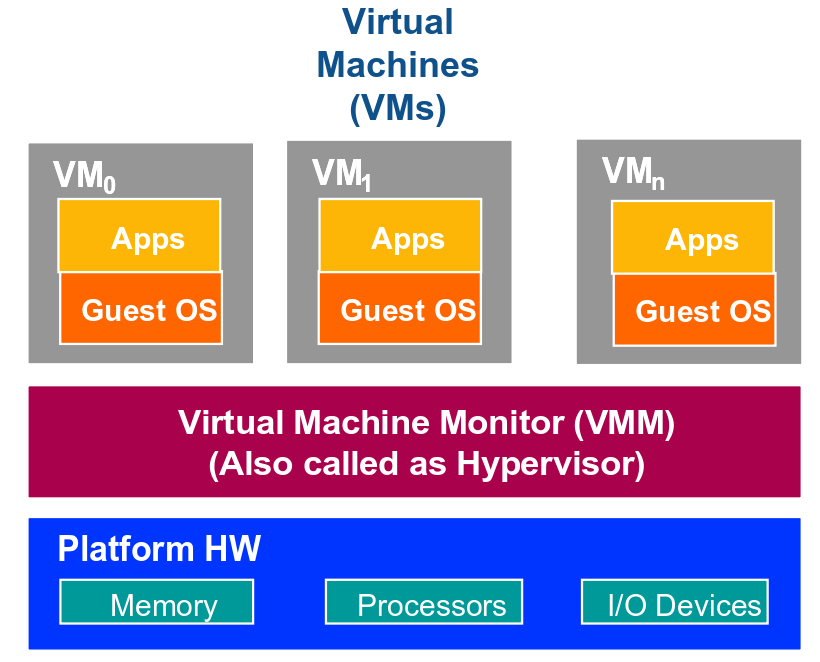
\includegraphics[width=1.\textwidth]{vmm-overview}
			
		\end{column}
		
		\begin{column}{.6\textwidth}
			
		\Large
		Before optimization of VMM ...
		\begin{itemize}
			\item Where is the bottlenecks of VMM?
			\item How to find these bottlenecks?
			
		\end{itemize} 	
			


		\end{column}
		
		
	\end{columns}
	
	
\end{frame}

%-------------------------------------------------
\begin{frame}[plain]
	\frametitle{Introduction -- Where is the bottlenecks of VMM?}



	\begin{columns}

	\begin{column}{.4\textwidth}
	
	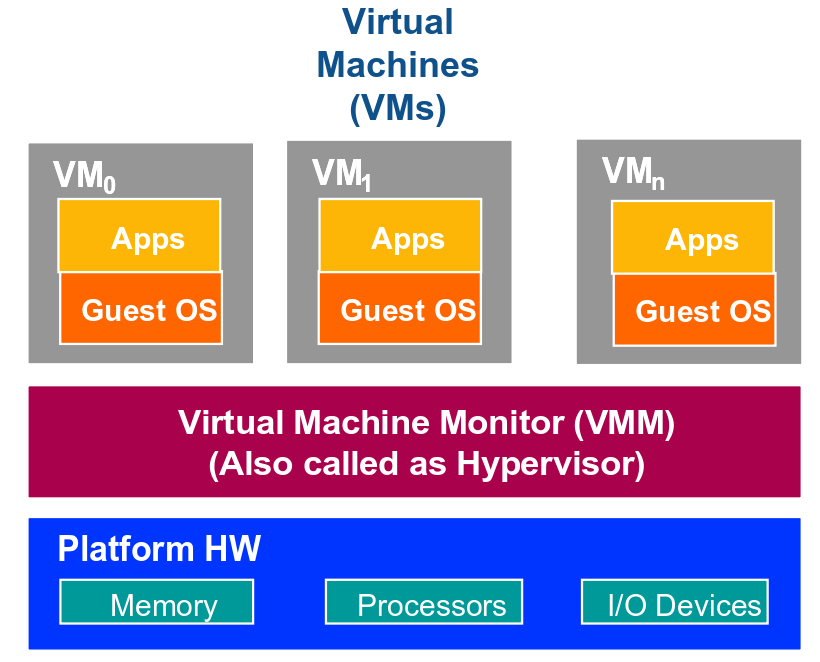
\includegraphics[width=1.\textwidth]{vmm-overview}
	
	\end{column}

	\begin{column}{.6\textwidth}
	
	\Large
    bottlenecks of VMM	
	\begin{itemize}
	\item VCPU
	\item VMEM
	\item VIO
	\item  etc...
	\end{itemize}	


	\end{column}
	
    
\end{columns}


\end{frame}


%-------------------------------------------------
\begin{frame}[plain]
	\frametitle{Introduction -- bottlenecks of VMM}
	
	
	
	\begin{columns}
		
		\begin{column}{.4\textwidth}
			\centering
			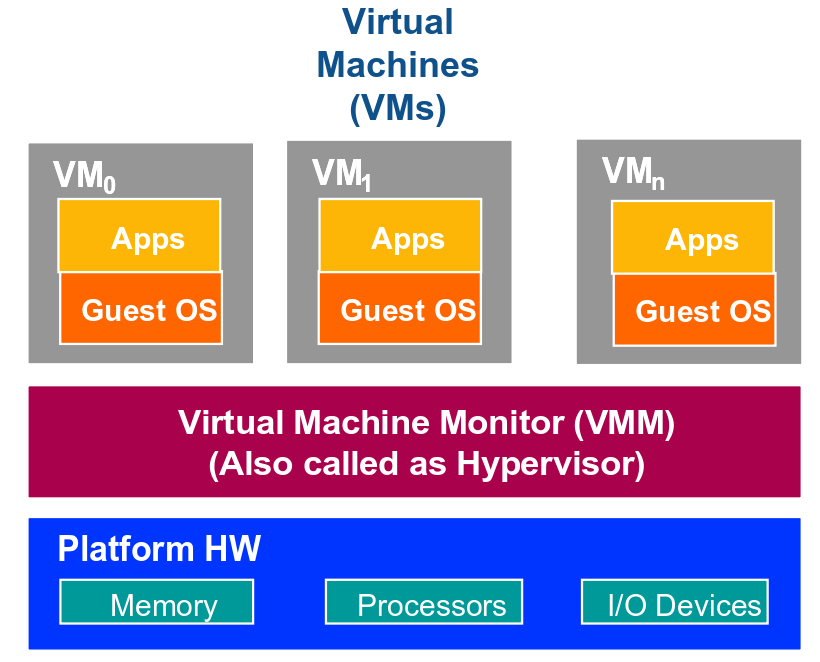
\includegraphics[width=.7\textwidth]{vmm-overview}
			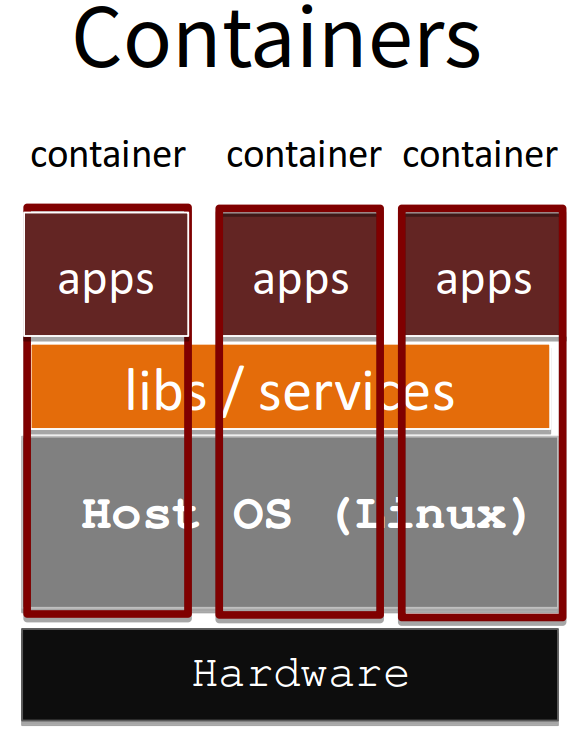
\includegraphics[width=.6\textwidth]{container-overview}
		\end{column}
		
		\begin{column}{.6\textwidth}
			
			\Large
			Comparison between VMM and Container
			\begin{itemize}
				\item Target: Docker v.s. KVM/XEN 
				\item Benchmark: Environment and Workload
				\item Testing \& Evaluation

			\end{itemize}	
			
			\tiny from: An Updated Performance Comparison of Virtual Machines	and Linux Containers,TR of IBM, 2014
			
			\tiny from: My VM is Lighter (and Safer) than your Container and Linux Containers,SOSO'17, 2017
		\end{column}
		
		
	\end{columns}
	
	
\end{frame}


%-------------------------------------------------
\begin{frame}[plain]
	\frametitle{Introduction -- Container overview }
	
	
	
	\begin{columns}
		
		\begin{column}{.3\textwidth}
			\centering

			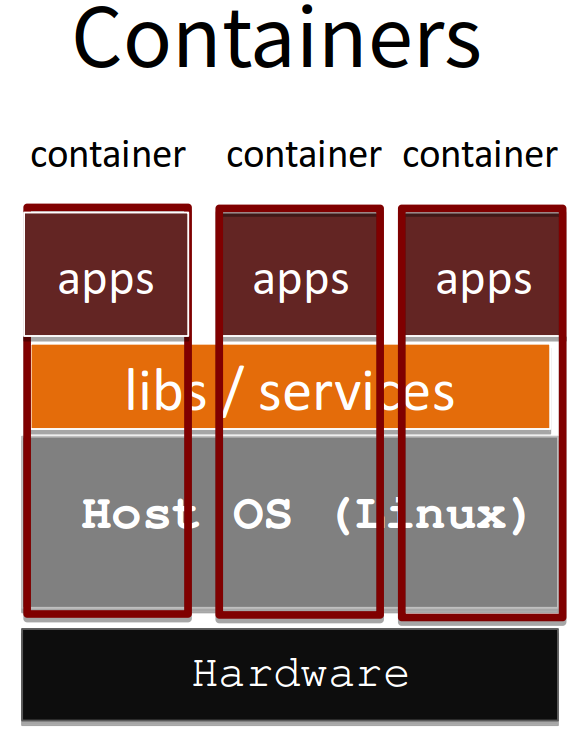
\includegraphics[width=1.\textwidth]{container-overview}
		\end{column}
		
		\begin{column}{.7\textwidth}
			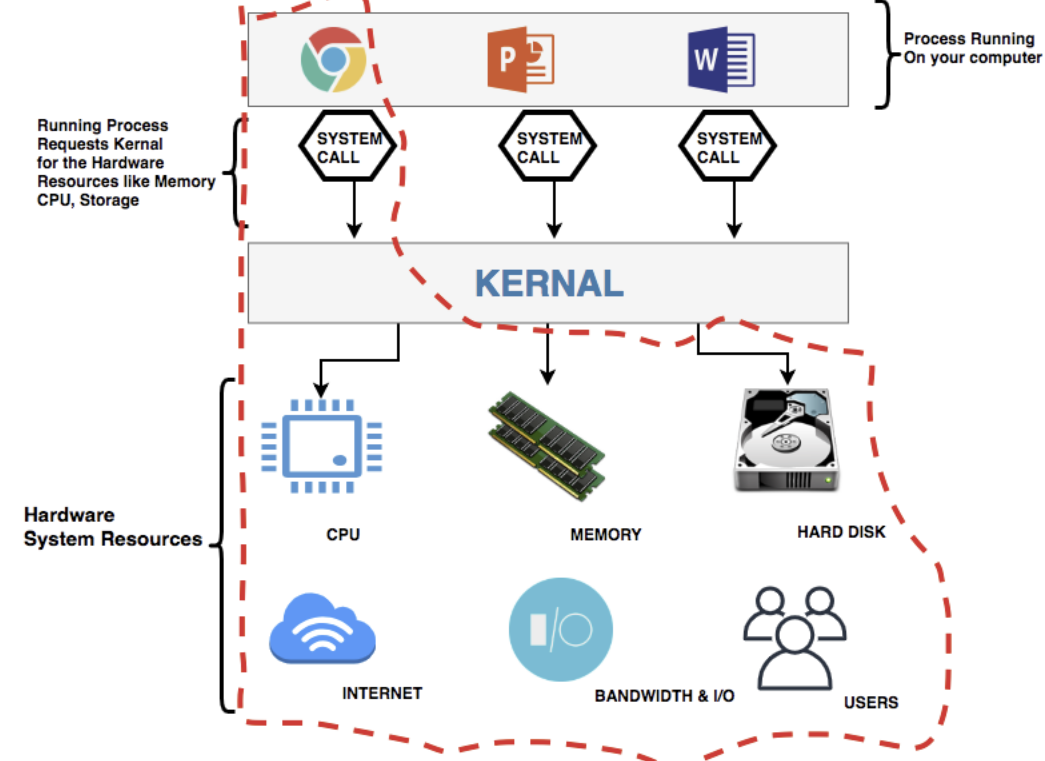
\includegraphics[width=1.\textwidth]{container-for-app}

		\end{column}
		
		
	\end{columns}
	
	
\end{frame}

%-------------------------------------------------
\begin{frame}[plain]
	\frametitle{Introduction -- Container overview }
	
	
	
	\begin{columns}
		
		\begin{column}{.3\textwidth}
			\centering
			
			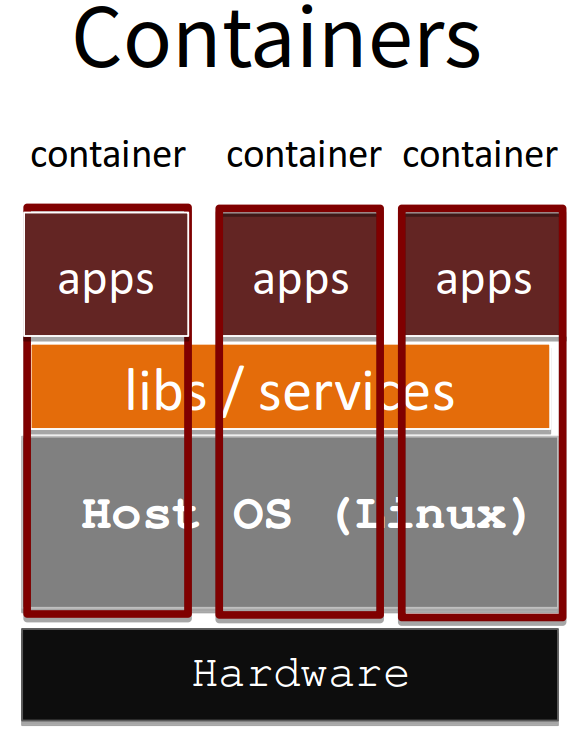
\includegraphics[width=1.\textwidth]{container-overview}
		\end{column}
		
		\begin{column}{.7\textwidth}
			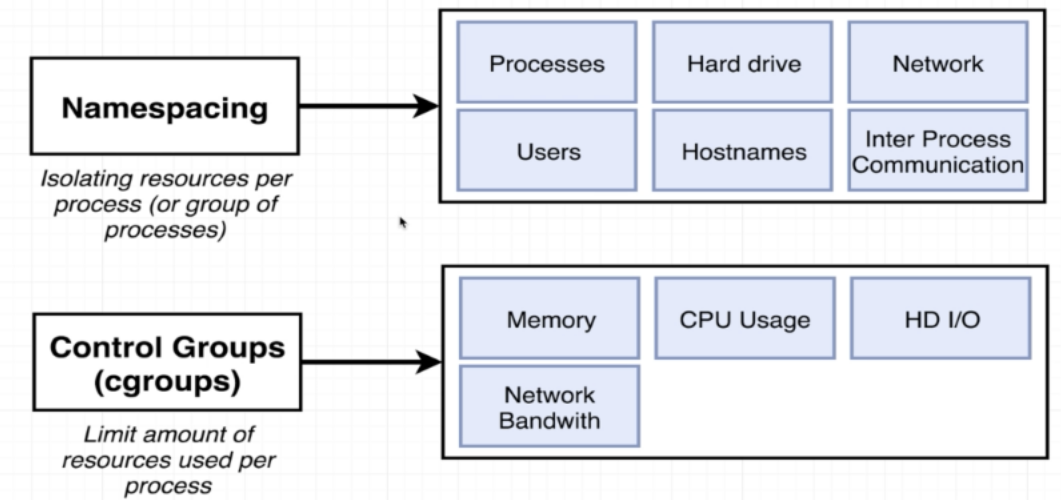
\includegraphics[width=1.\textwidth]{container-in-kernel}
			
		\end{column}
		
		
	\end{columns}
	
	
\end{frame}
%-------------------------------------------------

%-------------------------------------------------
\begin{frame}[plain]
	\frametitle{Introduction -- Container overview }
	
%	https://www.middlewareinventory.com/blog/what-is-container-and-containerization-a-basic-notes/
	
	\begin{columns}
		
		\begin{column}{.4\textwidth}
			\centering
			
			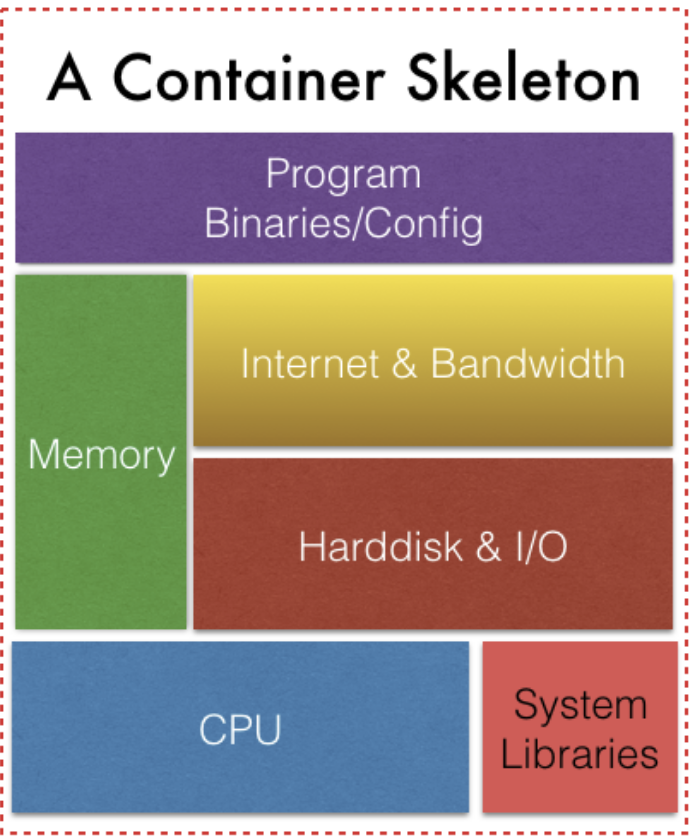
\includegraphics[width=1.\textwidth]{container-skeleton}
		\end{column}
		
		\begin{column}{.6\textwidth}
			\Large
			What is inside a Container
			\begin{itemize}
				\item Program Binaries/configuration
				\item Runtime libraries
				\item Dependency Products/tools
				\item A Piece of Kernal
				\item System Resources: CPU/MEM/IO/Net/Storage
				
			\end{itemize}	
			We are isolating the program and delicately providing its own system resources and runtime libraries.
		\end{column}
		
%		Docker is a container management system that helps us to efficiently manage Linux Containers (LXC) in a more comfortable and universal fashion.
	\end{columns}
	
	
\end{frame}

%-------------------------------------------------
\begin{frame}[plain]
	\frametitle{Introduction -- bottlenecks of VMM -- CPU/MEM}
	
			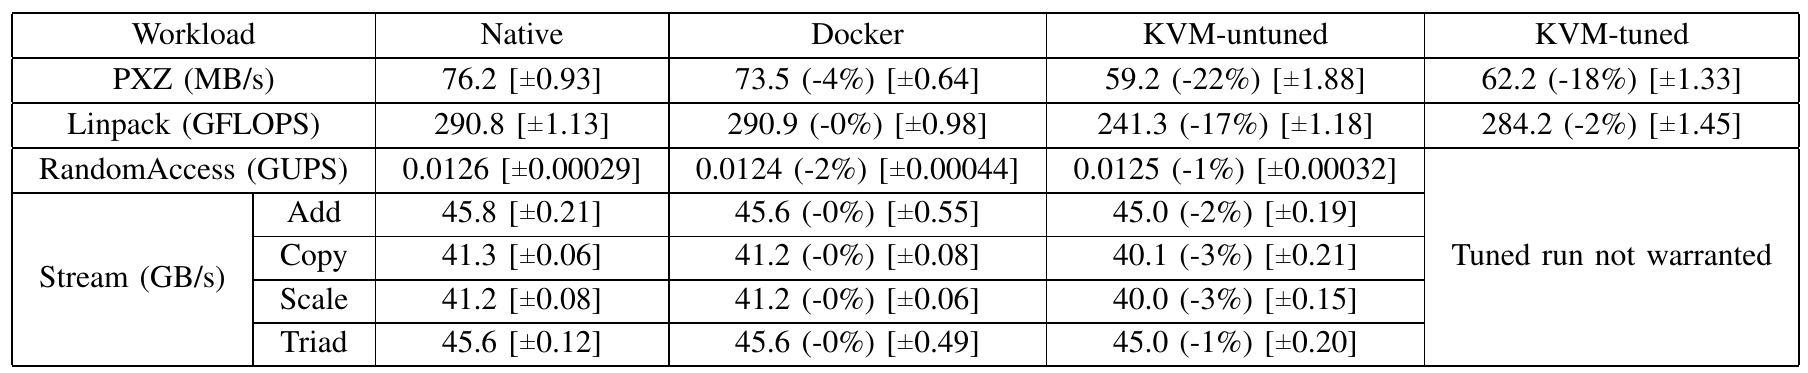
\includegraphics[width=1.\textwidth]{benchs-for-vmm-container}


			\large
			Environment
			\begin{itemize}
				\item two E5-2665 (16 cores with HT),  256 GB of RAM
				\item Direct 10 Gbps Ethernet link between
				two Mellanox ConnectX-2 EN NICs
				\item Ubuntu 13.10, kernel 3.11, Docker 1.0, QEMU 1.5.0
				\item 32vCPU (Power management was disabled)
			\end{itemize}	
	
\end{frame}


%-------------------------------------------------
\begin{frame}[plain]
	\frametitle{Introduction -- bottlenecks of VMM -- CPU/MEM}
	
	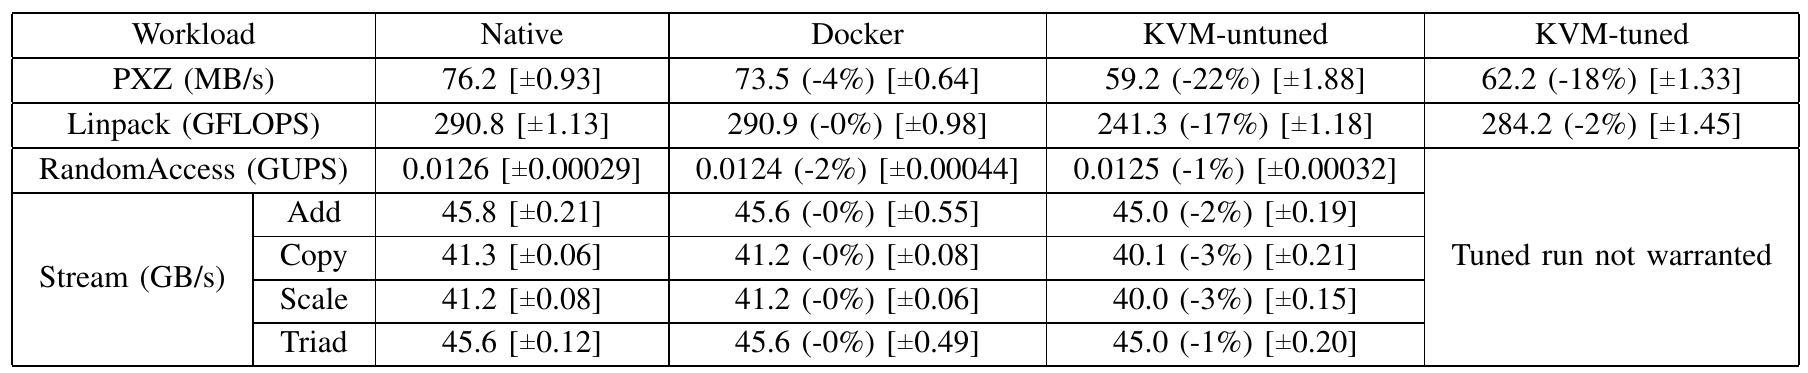
\includegraphics[width=1.\textwidth]{benchs-for-vmm-container}
	
	
	\large
	Results
	\begin{itemize}
		\item PXZ: extra TLB pressure of nested paging.
		\item Linpack:  pin vCPUs--> pCPU, expose the underlying
		cache topology
		\item STREAM: bandwidth of mem, cost of handling TLB misses, uses large pages
		
		
	\end{itemize}	
	\centering
	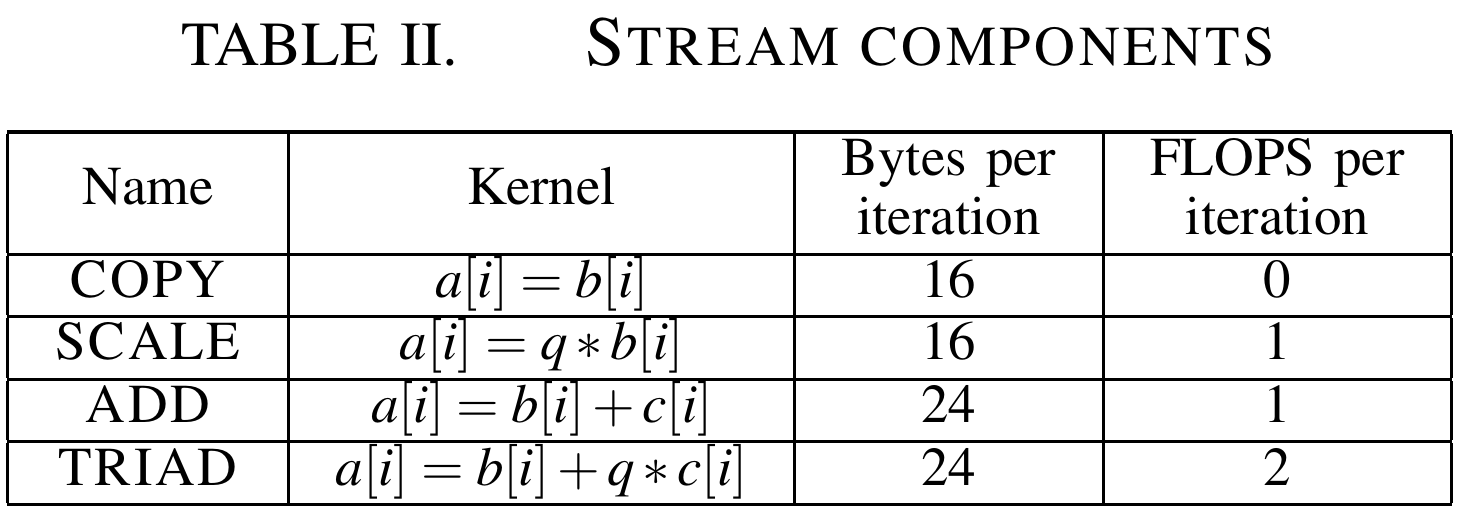
\includegraphics[width=.4\textwidth]{bench-stream}
\end{frame}
%-------------------------------------------------


%-------------------------------------------------
\begin{frame}[plain]
	\frametitle{Introduction -- bottlenecks of VMM -- Net }
	
	
	
	\begin{columns}
		
		\begin{column}{.4\textwidth}
%			\centering
			
			Network configurations
			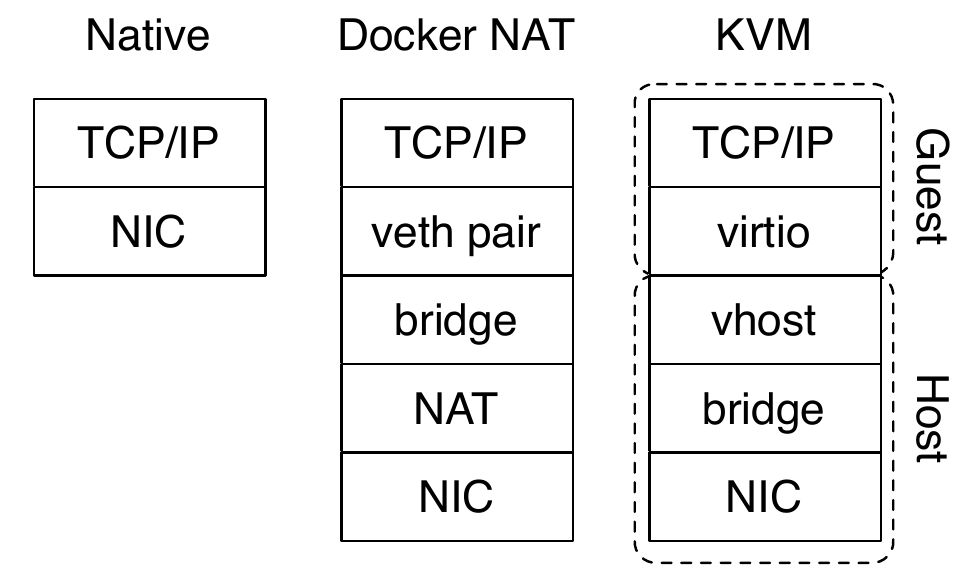
\includegraphics[width=1.\textwidth]{net-config}
			
			
			\small
		     nuttcp to measure network bandwidth
			\begin{itemize}
			\item  All three configurations reach 9.3 Gbps
			\item NAT noticeably increases overhead
			\item vhost reduces overhead 
%			\item all have heavy overhead for latency
			\item NIC is the bottleneck
			
			\end{itemize}
		
		\end{column}
		
		\begin{column}{.6\textwidth}
			\centering
			TCP bulk transfer efficiency (CPU cycles/byte)
			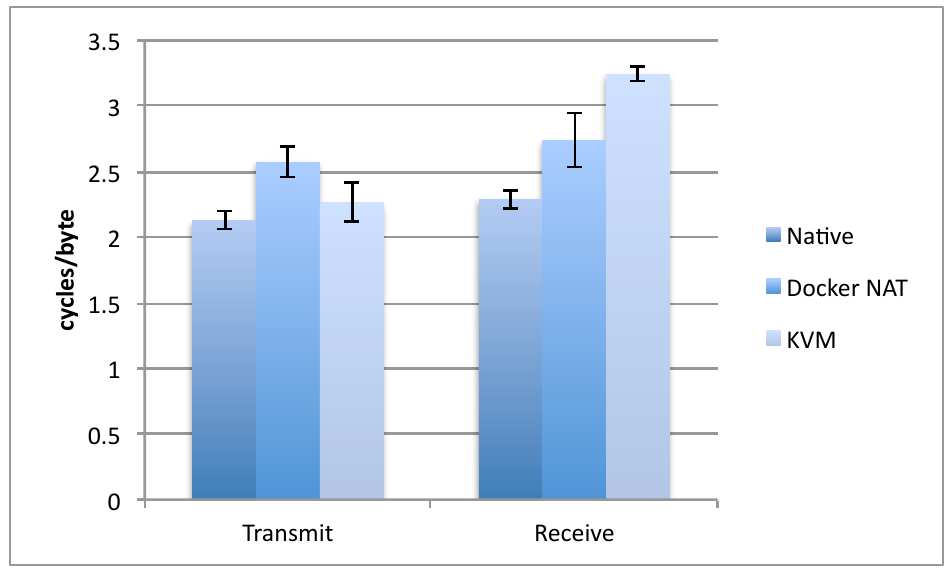
\includegraphics[width=.6\textwidth]{tcp-bulk-transfer}
			
			Network round-trip latency (μs)
			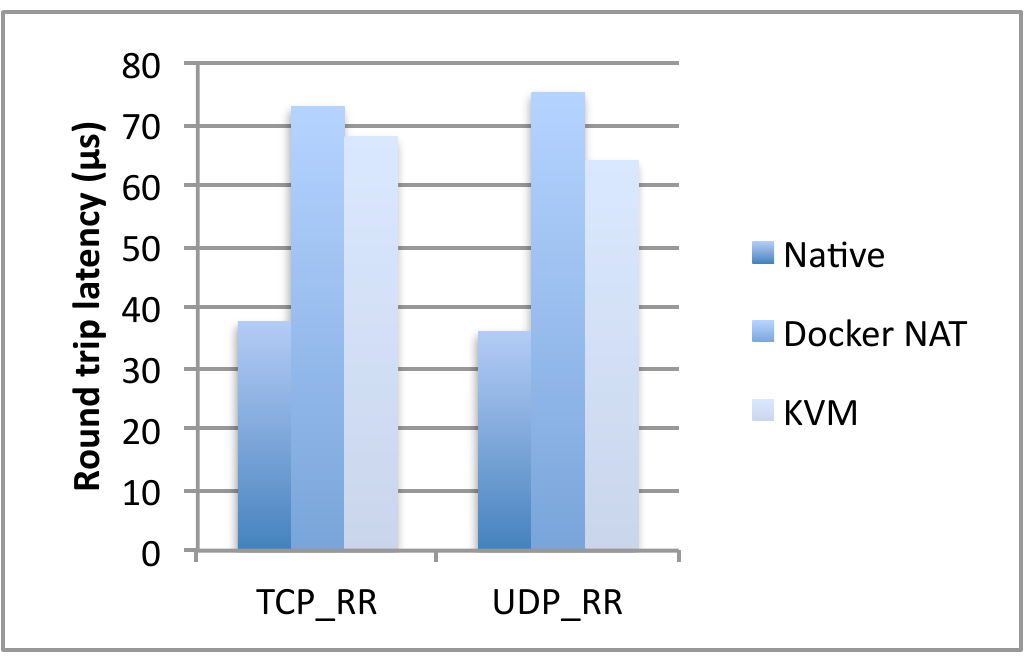
\includegraphics[width=.6\textwidth]{net-roundtrip-latency}
		\end{column}
		
		
	\end{columns}
	
	
\end{frame}




%-------------------------------------------------
\begin{frame}[plain]
	\frametitle{Introduction -- bottlenecks of VMM -- Storage }
	
	
	
	\begin{columns}
		
		\begin{column}{.4\textwidth}
			%			\centering
			
			Storage configurations
			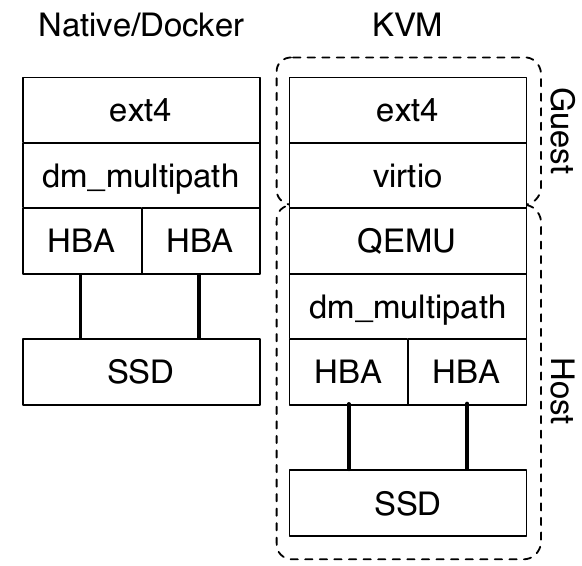
\includegraphics[width=.6\textwidth]{storage-config}
			
			
			\small
			
			\begin{itemize}
			\item  20 TB SSD, two 8 Gbps Fibre Channel links
			\item  fio with the	libaio backend in O DIRECT mode 
			\item Fibre Channel HBA is the bottleneck

				
			\end{itemize}
			
		\end{column}
		
		\begin{column}{.6\textwidth}
			\centering
			Sequential I/O throughput (MB/s)
			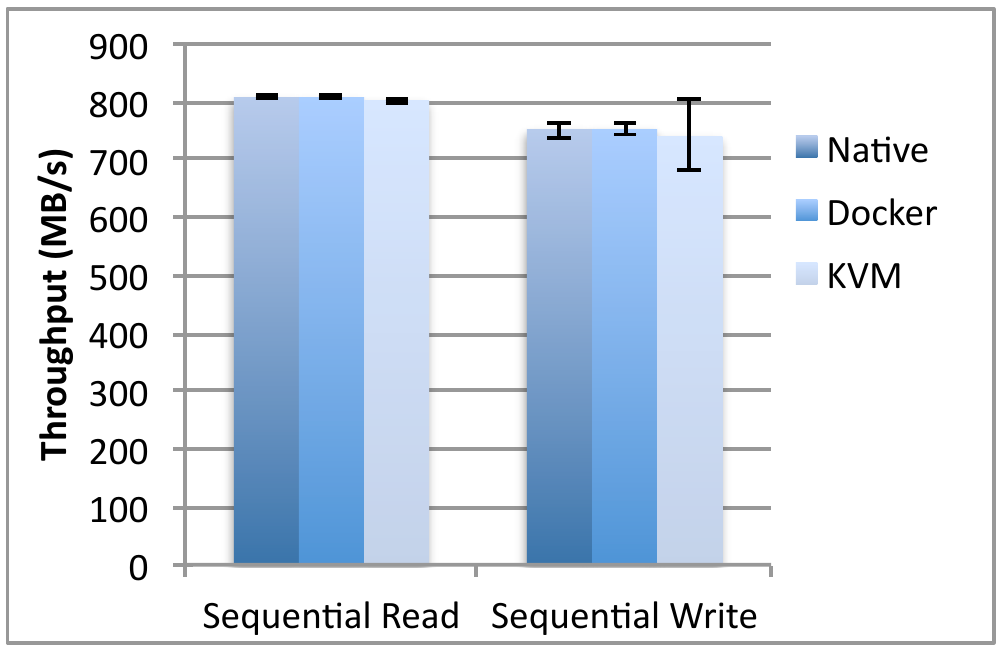
\includegraphics[width=.6\textwidth]{bench-store-seq}
			
			 Random I/O throughput (IOPS)
			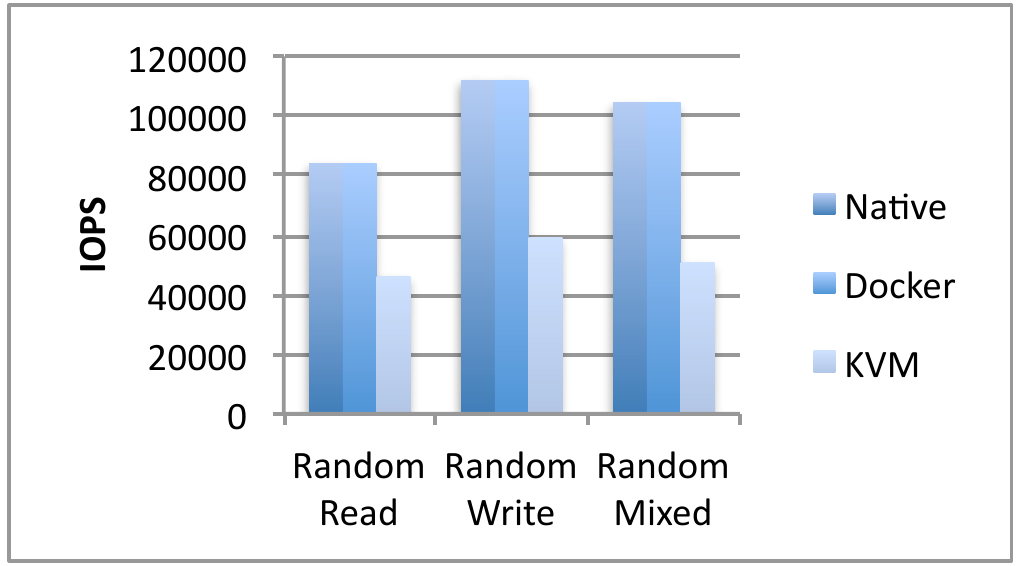
\includegraphics[width=.6\textwidth]{bench-store-rand}
		\end{column}
		
		
	\end{columns}
	
	
\end{frame}


%-------------------------------------------------
\begin{frame}[plain]
	\frametitle{Introduction -- bottlenecks of VMM -- Real Apps }
	
	
	
	\begin{columns}
		
		\begin{column}{.5\textwidth}
						\centering
			
			MySQL configurations
			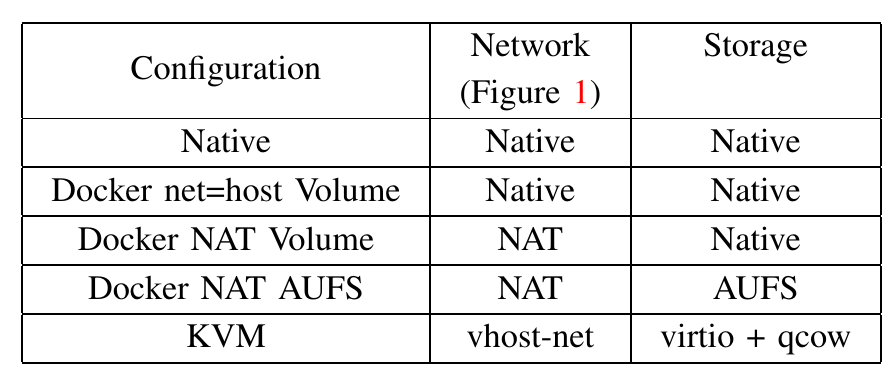
\includegraphics[width=.8\textwidth]{mysql-config}
			
			MySQL throughput (transactions/s)
			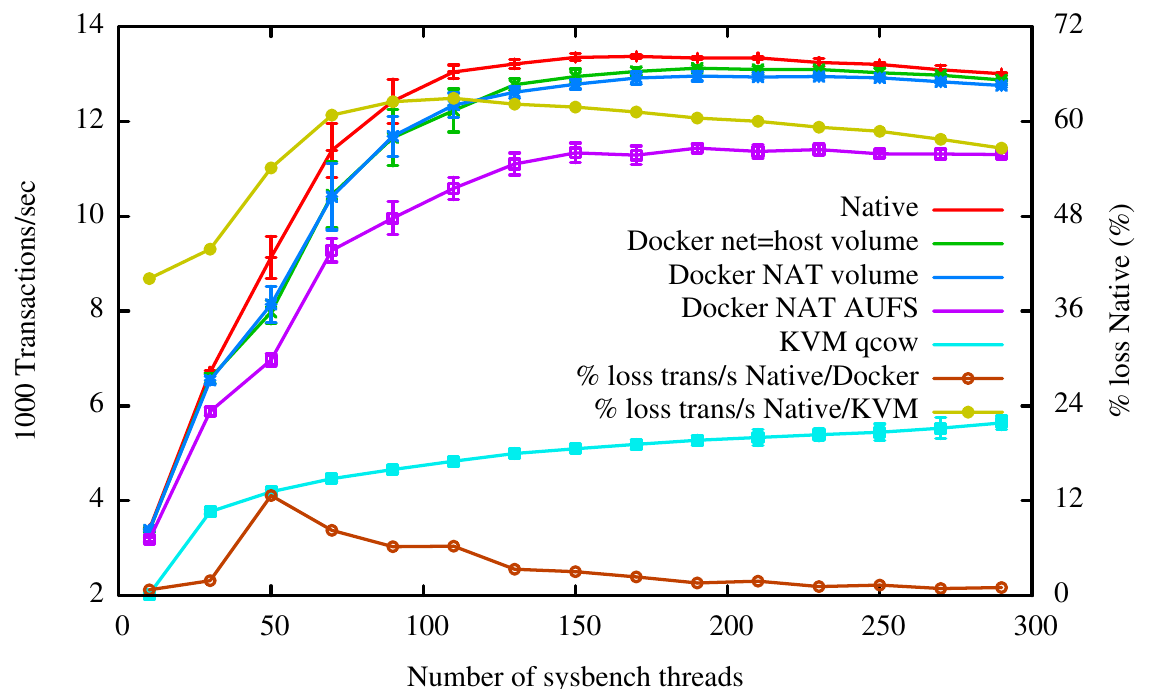
\includegraphics[width=.8\textwidth]{mysql-throughput}
			\small

			
		\end{column}
		
		\begin{column}{.5\textwidth}
			\centering
			Redis performance (requests/s) 
			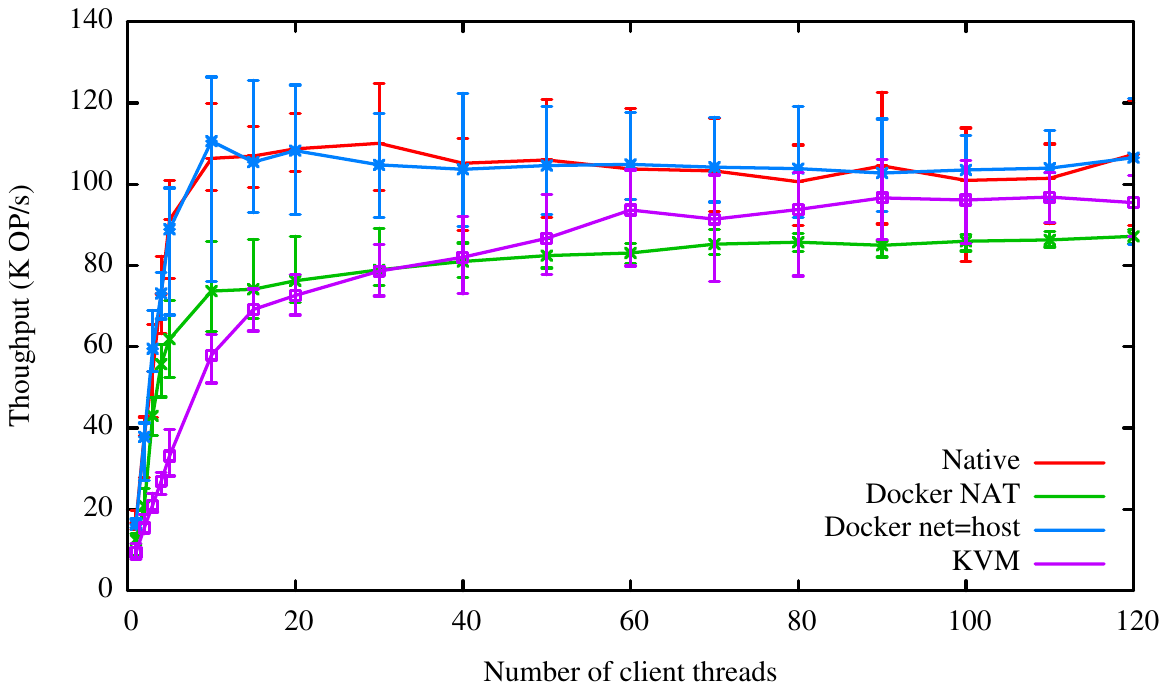
\includegraphics[width=.7\textwidth]{redis-perf}
			
			Average latency (in ms) of operations on  Redis
			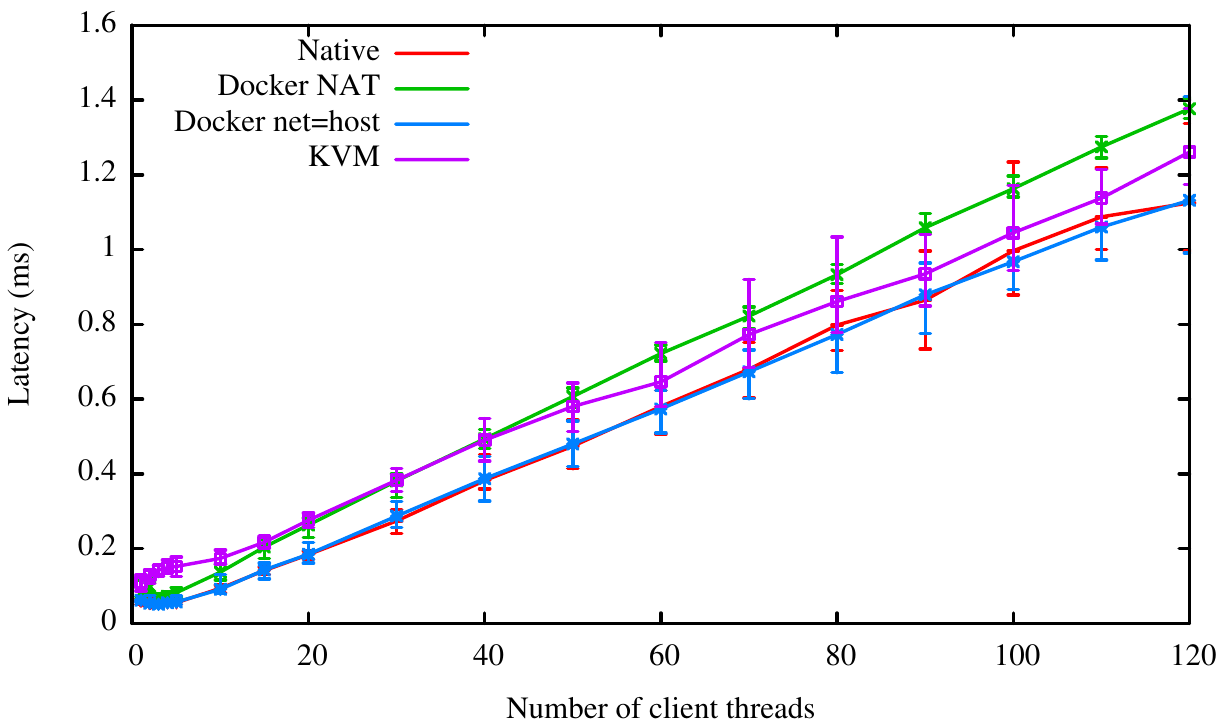
\includegraphics[width=.7\textwidth]{redis-latency}
		\end{column}
		
		
	\end{columns}
	
	
\end{frame}


%-------------------------------------------------
\begin{frame}[plain]
	\frametitle{Introduction -- bottlenecks of VMM -- Summary}
	
	
	
	\begin{columns}
		
		\begin{column}{.4\textwidth}
			\centering
			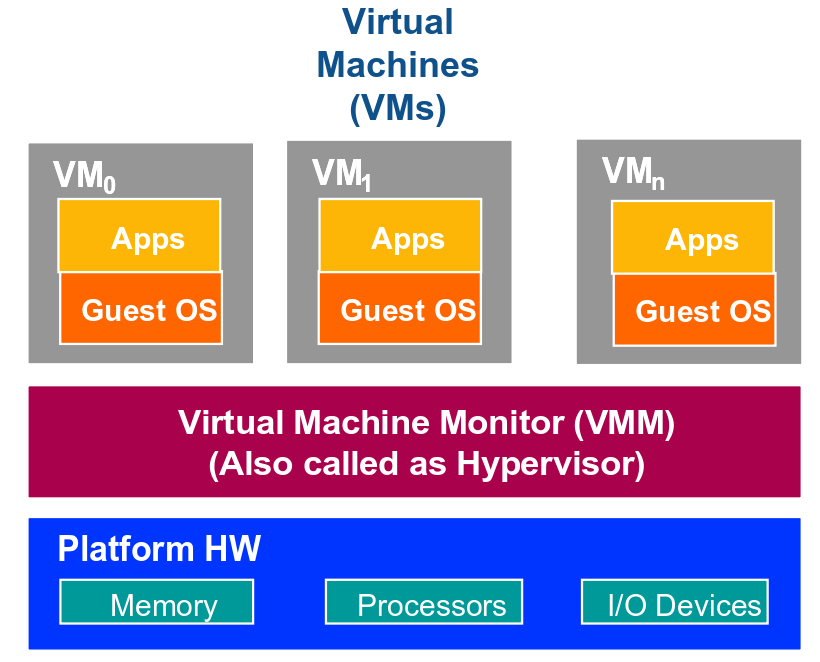
\includegraphics[width=.7\textwidth]{vmm-overview}
			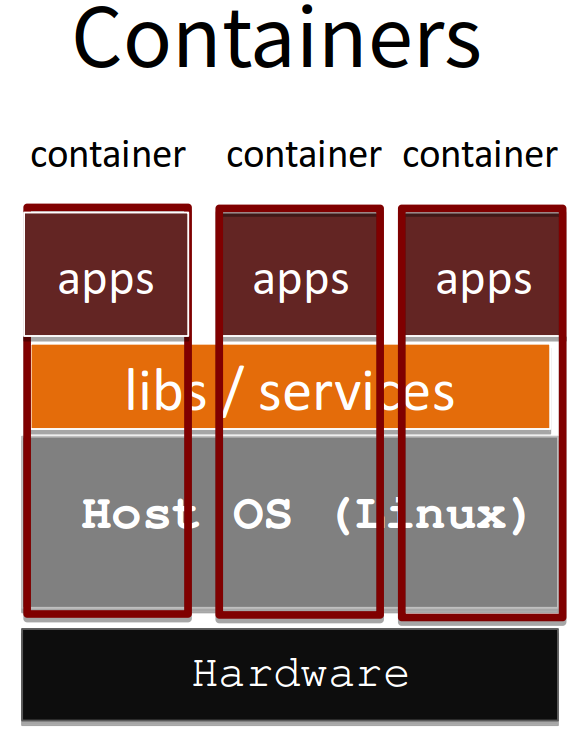
\includegraphics[width=.6\textwidth]{container-overview}
		\end{column}
		
		\begin{column}{.6\textwidth}
			
%			\Large
			Summary
			\begin{itemize}
				\item Containers and VMs impose almost
				no overhead on CPU and memory usage; they only impact
				\underline{I/O and OS interaction}. 
				\item This overhead comes in the form of
				extra cycles for each I/O operation, so small I/Os suffer much
				more than large ones. 
				\item Several additional topics worthy of investigation: 
				\underline{performance isolation}
				when multiple workloads run on the same server, live resizing
				of containers and VMs, tradeoffs between scale-up and scale-
				out, and tradeoffs between live migration and restarting.
				
				\item https://github.com/thewmf/kvm-docker-comparison
				
			\end{itemize}	
			
		\end{column}
		
		
	\end{columns}
	
	
\end{frame}
%-------------------------------------------------
%-------------------------------------------------
\end{document}